\documentclass[aspectratio=169]{beamer}
\usepackage[utf8]{inputenc}
\usepackage{amsmath}
\usepackage{amssymb}
\usepackage{amsfonts}
\usepackage{dsfont}
\usepackage{tikz}
\usepackage{pgfplots}
\usepackage{opensans}

\usetikzlibrary{shapes,arrows,positioning}
\pgfplotsset{compat=1.8,samples=25}

\usetheme{NOVASBE}

\title[]{4509 - Bridging Mathematics}
\subtitle{Markov Chains}
\author[P. Fagandini]{Paulo Fagandini}
\institute{}
\date{}

\newtheorem{defenition}{Definition}[section]
\newtheorem{proposition}{Proposition}[section]
\newtheorem{conjecture}{Conjecture}[section]

\begin{document}

\begin{frame}{Discrete-time Markov chains}
    \begin{enumerate}
        \item Time is indexed by an integer variable, say $n$.
        \item At period $n$, the \textbf{state} of the chain is denoted by $X_{n\cdot}$.
        \item $\mathcal{S}$ is a finite set of possible states, then $X_n\in\mathcal{S}$.
        \item We will allow for $m$ different states, then $\mathcal{S}=\{1,2,\hdots,m\}$, for $m\in\mathds{N}$.
    \end{enumerate}
\end{frame}

\begin{frame}{Discrete-time Markov chains}
    \begin{definition}{Markov Chain}
        The Markov chain is described in terms of its \textbf{transition probabilities} $p_{ij}$:
        whenever the state happens to be $i$, there is probability $p_{ij}$ that the next state is
        equal to $j$:
        \[p_{ij}=P(X_{n+1}=j|X_n=i), \quad i,j\in\mathcal{S}\]
        with $p_{ij}\geq 0$ and $\sum_{j=1}^m p_{ij}=1$ $\forall i$.
    \end{definition}    

    \vspace{1em}

    \onslide<2->{
        \textbf{Note:} the probability does not depend on time, nor anything else than the present state.
    }
\end{frame}

\begin{frame}
    How to specify then a Markov Model?
    \begin{itemize}
        \item Identify:
            \begin{enumerate}
                \item $\mathcal{S}$ the set of states.
                \item the set of possible transitions, $(i,j)$ where $p{ij}>0$
                \item the values for those $p_{ij}$
            \end{enumerate}
        \item The Markov chain specified by this model is a sequence of r.v.s $X_0,X_1,X_2,\hdots$, that
              can take values in $\mathcal{S}$, and which satisfy:
              \[P(X_{n+1}=j|X_n=i, \{X_{\nu}=i_{\nu}\}_{\nu=0}^{n-1})=p_{ij}\] for any $n$, and any $i,j\in\mathcal{S}$,
              and all possible sequences $i_0,\hdots,i_{n-1}$ of earlier states.
    \end{itemize}
\end{frame}

\begin{frame}
    It is convenient to sort all these probabilities in a two-dimensional array like this:
    \begin{align*}
        \begin{bmatrix}
            p_{11}&p_{12}&\hdots&p_{1m}\\
            p_{21}&p_{22}&\hdots&p_{2m}\\
            \vdots&\vdots &\ddots & \vdots\\
            p_{m1}&p_{m2}&\hdots&p_{mm}
        \end{bmatrix}
    \end{align*}
    This is called the \textbf{Transition Probability Matrix}. This matrix is defined as having in each
    row $i$ and column $j$ the probability of transitioning from state $i$ to state $j$.
\end{frame}

\begin{frame}{Example, Bertsekas and Tsitsiklis (2008)}
    Alice is taking a probability class and in each week, she can be
    either up-to-date or she may have fallen behind. If she is up-to-date in a given
    week, the probability that she will be up-to-date (or behind) in the next week is
    $0.8$ (or $0.2$, respectively) . If she is behind in the given week, the probability that
    she will be up-to-date (or behind) in the next week is $0.6$ (or $0.4$, respectively) . We
    assume that these probabilities do not depend on whether she was up-to-date or
    behind in previous weeks, so the problem has the typical Markov chain character
    (the future depends on the past only through the present)
\end{frame}

\begin{frame}
    Let $1$ be the state of being up-to-date and $2$ that she fell behind.

    \vspace{0.5em}
    \onslide<2->{
        The transition probabilities:
        {
            \centering
            \begin{tabular}{cccc}
                $p_{11}=0.8$ & $p_{12}=0.2$ & $p_{21}=0.6$ & $p_{22}=0.4$
            \end{tabular}
        }
    }

    \vspace{0.5em}

    \onslide<3->{
        The transition probability matrix:
        \begin{align*}
            \begin{bmatrix}
                0.8 & 0.2 \\
                0.6 & 0.4 
            \end{bmatrix}
        \end{align*}
    }


\end{frame}

\begin{frame}
        The transition probability graph:

        \vspace{0.5em}

        \begin{center}
            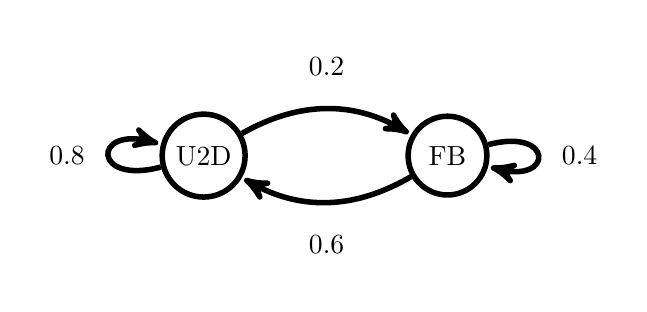
\begin{tikzpicture}[
                scale=0.5,
                ->,
                >=stealth',
                shorten >=1pt,
                line width=2pt, 
                node distance=2cm,
                style ={minimum size=10mm},
                every node/.style={scale=0.6}]

                \tikzstyle{every node}=[font=\normalsize]

                \node [circle, draw] (a) {U2D};
                \path  (a) edge [loop left] node[midway,left,inner sep=2pt] {0.8} (a);

                \node [circle, draw] (b) [right=of a] {FB};
                \path  (b) edge [loop right] node[midway,right,inner sep=2pt] {0.4} (b);
                
                \draw[->] (a) to[bend left] node[midway,above,inner sep=2pt] {0.2} (b);
                \draw[->] (b) to[bend left] node[midway,below,inner sep=2pt] {0.6} (a);


            \end{tikzpicture}
        \end{center}
    

\end{frame}

\begin{frame}
    We have said that the state today depends only on the state in the previous period.
    This is true, however, we can get around this constraint.
    
    \vspace{1em}

    Consider the following example:
    \begin{enumerate}
        \item A working machine can be working the next day with probability $p$, and be broken with probability $1-p$.
        \item A broken machine can be working the next day with probability $q$, and remain broken with probability $1-q$.
    \end{enumerate}

    \vspace{1em}

    However, what happens if the machine cannot be fixed for, say, 4 straight days? Maybe we need to buy a new one. To model this
    we can introduce new states to our system.

\end{frame}

\begin{frame}
    \begin{enumerate}
        \item A working machine can be working the next day with probability $p$, and be 1-day broken with probability $1-p$, and zero for $n$-days broken for $n>1$.
        \item A 1-day broken machine can be working the next day with probability $q$, and become 2-day broken with probability $1-q$, and zero for $n$-days broken for $n\neq2$.
        \item A 2-days broken machine can be working the next day with probability $r$, and become broken for 3 days with probability $1-r$, and zero for $n$-days broken for $n\neq3$.
        \item A 3-days broken machine can be working the next day with probability $s$, and become broken for 4 days with probability $1-s$, and zero for $n$-days broken for $n\neq4$.
        \item A 4-days broken machine can be working with probability $1$, and zero for all the other broken states.
    \end{enumerate}

\end{frame}

\begin{frame}
    \begin{definition}[$n$-Step Transition Probabilities]
        Let $r_{ij}(n)$ represent the probability that the state after $n$ time periods will be $j$, given that the current state is $i$.
        \[r_{ij}(n)=P(X_n=j|X_0=i)\]
    \end{definition}
    \begin{proposition}[Chapman-Kolmogorov]
        The n-step transition probabilities can be generated by the recursive formula:
        \[r_{ij}(n)=\sum_{k=1}^m r_{ik}(n-1)p_{kj},\quad \text{for\ }n>1,\ \text{and all }i,j\]
        starting with \[r_{ij}(1)=p_{ij}\]
    \end{proposition}
    
\end{frame}

\begin{frame}
    Note that this is an element of the following matrix:
    \begin{align*}
        \begin{bmatrix}
            p_{11}&p_{12}&\hdots&p_{1m}\\
            p_{21}&p_{22}&\hdots&p_{2m}\\
            \vdots&\vdots &\ddots & \vdots\\
            p_{m1}&p_{m2}&\hdots&p_{mm}
        \end{bmatrix}^n
    \end{align*}
\end{frame}

\begin{frame}
    This ``realization'' allow us to be able to ask and answer some interesting questions:
    \begin{itemize}
        \item What can we say about limits? What happens as $n\rightarrow\infty$?
        \item The dependence of the state at $n$ over the initial state becomes smaller as $n$ increases.
        \item What can we say qualitatively about the behavior of this markov chain?
    \end{itemize}
\end{frame}

\begin{frame}
    Consider the transition matrix for the example we just saw:
    \begin{align*}
        A=\begin{bmatrix}
            0.8 & 0.2 \\
            0.6 & 0.4 
        \end{bmatrix}\quad
        \onslide<2->{
            &A^2&=\begin{bmatrix}
                0.7600 & 0.2400 \\
                0.7200 & 0.2800 
            \end{bmatrix}&\quad
        }
        \onslide<3->{
            &A^3&=\begin{bmatrix}
                0.7520 & 0.2480 \\
                0.7440 & 0.2560 
            \end{bmatrix}&\\
        }
        \onslide<4->{
            &A^4&=\begin{bmatrix}
                0.7504 & 0.2496 \\
                0.7488 & 0.2512 
            \end{bmatrix}&\quad
        }
        \onslide<5->{
            &A^5&=\begin{bmatrix}
                0.7501 & 0.2499 \\
                0.7498 & 0.2502 
            \end{bmatrix}&\\
        }
        \onslide<6->{
            &A^6&=\begin{bmatrix}
                0.7500 & 0.2500 \\
                0.7500 & 0.2500 
            \end{bmatrix}&\quad
        }
        \onslide<7->{
            &A^7&=\begin{bmatrix}
                0.7500 & 0.2500 \\
                0.7500 & 0.2500 
            \end{bmatrix}&
        }
    \end{align*}
    Note how as $n\rightarrow\infty$ $r_{ij}(n)$ goes to a limit that does not depend on the initial state.
\end{frame}

\begin{frame}
    \begin{definition}[Accessible state]
        A state $j$ is accessible from a state $i$ if $\exists n\in\mathds{N}$ such that the $n$-step 
        transition probability $r_{ij}(n)$ is positive, i.e., if there is positive probability of reaching
        $j$, starting from $i$, after some number of periods.
    \end{definition}
    \onslide<2->{
    \begin{definition}[Recurrent state]
        Let $A(i)$ be the set of states that are accessible from $i$. We say that $i$ is \textbf{recurrent}
        if $\forall j\in A(i) \Rightarrow i\in A(j)$.
    \end{definition}
    }
    \onslide<3->{
    \begin{definition}[Transient state]
        A state is called \textbf{transient} if it is not recurrent.
    \end{definition}
    }
\end{frame}

\begin{frame}
    \begin{corollary}
        A recurrent state will be visited an infinity amount of times.
    \end{corollary}

    \begin{corollary}
        A transient state will be visited a finite amount of times.
    \end{corollary}
\end{frame}

\begin{frame}
    Which of the following nodes are transient and which are recurrent?

    \vspace{0.5em}

    \begin{center}
        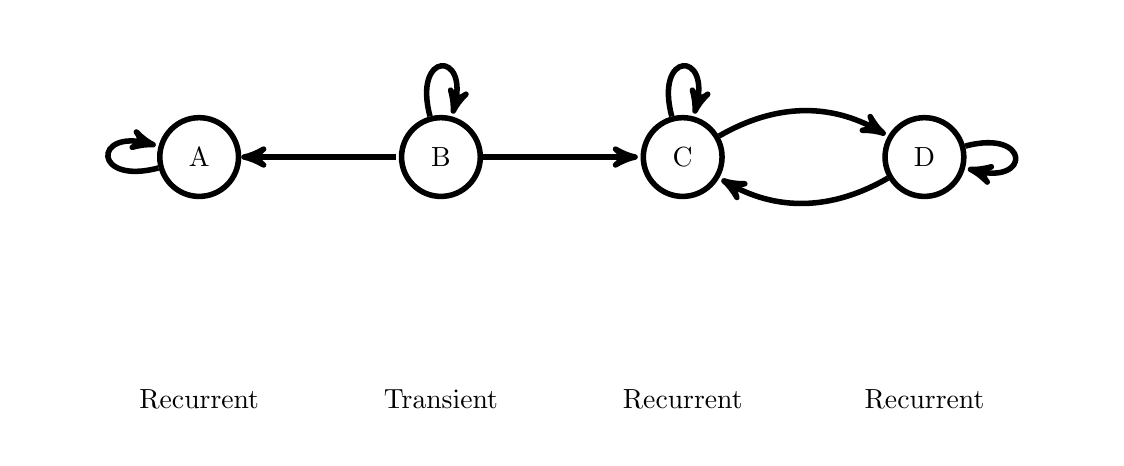
\begin{tikzpicture}[
            scale=0.5,
            ->,
            >=stealth',
            shorten >=1pt,
            line width=2pt, 
            node distance=2cm,
            style ={minimum size=10mm},
            every node/.style={scale=0.6}]

            \tikzstyle{every node}=[font=\normalsize]

            \node [circle, draw] (a) {A};
            \path  (a) edge [loop left] node[midway,left,inner sep=2pt] {} (a);

            \node [circle, draw] (b) [right=of a] {B};
            \path  (b) edge [loop above] node[midway,right,inner sep=2pt] {} (b);

            \node [circle, draw] (c) [right=of b] {C};
            \path  (c) edge [loop above] node[midway,right,inner sep=2pt] {} (c);

            \node [circle, draw] (d) [right=of c] {D};
            \path  (d) edge [loop right] node[midway,right,inner sep=2pt] {} (d);
            
            \draw[<-] (a) -- (b);
            \draw[->] (b) -- (c);
            \draw[->] (c) to[bend left] node[midway,above,inner sep=2pt] {} (d);
            \draw[->] (d) to[bend left] node[midway,below,inner sep=2pt] {} (c);

            \onslide<2->{
                \node [below=of a] {Recurrent};
            }
            \onslide<3->{
                \node [below=of b] {Transient};
            }
            \onslide<4->{
                \node [below=of c] {Recurrent};
            }
            \onslide<5->{
                \node [below=of d] {Recurrent};
            }

        \end{tikzpicture}
    \end{center}

\end{frame}

\begin{frame}
    \begin{definition}[Recurrent class]
        If $i$ is a recurrent state, the set of sattes $A(i)$ that are accessible from $i$ form a
        \textbf{recurrent class} (or simply a class), meaning that states in $A(i)$ are all accessible
        from each other, and no state outside $A(i)$ is accessible from them.
    \end{definition}
\end{frame}

\begin{frame}{Steady state behavior}
    When we talk about steady state in Markov Chains, it is not the ``state'' that is steady,
    but the probabilities of arriving to a certain state, remember the example we had before?
    \[\pi_j=P(X_n=j),\quad \text{ when } n \text{ is large.}\]
\end{frame}

\begin{frame}
    \begin{theorem}[Steady-State Convergence Theorem]
        Consider a Markov chain with a single recurrent class, which is periodic. Then, the states
        $j$ are associated with steady-state probabilities $\pi_j$ that have the following properties:
        \begin{enumerate}
            \item For each $j$, we have \[\lim_{n\rightarrow\infty}r_{ij}(n)=\pi_j,\quad\forall i\]
            \item The $\pi_j$ are the unique solution to the system of equations below:
                  \begin{align*}
                    \pi_j&=\sum_{k=1}^m\pi_{k}p_{kj},\quad j=1,\hdots,m,\\
                    1&= \sum_{k=1}^m \pi_k
                  \end{align*}
            \item We have
                  \begin{center}
                    \begin{tabular}{cl}
                        $\pi_j=0$&, for all transient states $j$\\
                        $\pi_j>0$&, for all recurrent states $j$
                    \end{tabular}
                  \end{center}
        \end{enumerate}
    \end{theorem}
\end{frame}

\begin{frame}
    Note that the steady-state probabilities add up to 1...\pause

    Therefore these form a probability distribution on the state space, this is called the
    \textbf{stationary distribution} of the chain.
\end{frame}

\begin{frame}
    \begin{definition}[Balance Equations]
        The equations \[\pi_j=\sum_{k=1}^m \pi_k p_{kj},\quad j=1,\hdots,m,\]
        are called \textbf{balance equations}, and they are a direct consequence of the first part
        of the Steady-State Convergence Theorem, and the Chapman-Kolmogorov equation.
    \end{definition}
    \begin{definition}[Normalization Equation]
        The equation \[sum_{k=1}^m \pi_k=1\] is known as the \textbf{normalization equation.}
    \end{definition}
\end{frame}

\begin{frame}{Example}
    Consider our original example:
    {    
        \centering
        \begin{tabular}{cccc}
            $p_{11}=0.8$ & $p_{12}=0.2$ & $p_{21}=0.6$ & $p_{22}=0.4$
        \end{tabular}
    }

    Clearly, on the limit $r_{ij}\rightarrow \pi_j$ if this converges, then the balance equations say:
    \begin{center}
    \begin{tabular}{cc}
        $\pi_1=\pi_1 p_{11}+\pi_2 p_{21}$ & $\pi_2=\pi_1 p_{12}+\pi_2 p_{22}$    
    \end{tabular}
    \end{center}

    Which, replacing, become:

    \begin{center}
    \begin{tabular}{cc}
        $\pi_1= 0.8 \pi_1 + 0.6 \pi_2$ & $\pi_2=0.2 \pi_1+0.4 \pi_2$    
    \end{tabular}
    \end{center}

    Solving, we obtain $\pi_1=3\pi_2$ in both equations, which together with the normalization equation
    $\pi_1+\pi_2=1$ lead us to:
    \begin{align*}
        \pi_1=0.75\\
        \pi_2=0.25
    \end{align*}

\end{frame}

\end{document}
